\chapter{Grid Information}
\label{chap:grid_information}

This chapter describes several of the MPAS grid variables and dimensions. The majority of these are common across all cores.

\section{Grid dimensions}

{\small
\begin{longtable}{|p{1.75in} |p{4.5in}|}
 \hline
        Time     &   netCDF record (unlimited) dimension \\ \hline
        nCells       &   Number of cells in the grid \\ \hline
        nEdges      &   Number of edges (cell faces) in the grid \\ \hline
        nVertices    &   Number of vertices (cell corners) in the grid \\ \hline
        nVertLevels     &   Number of vertical layers \\ \hline
        nVertLevelsP1   &   Number of vertical levels (nVertLevels + 1) \\ \hline
        maxEdges        &   Maximum number of neighbor cells of any cell \\ \hline
        maxEdges2       &   Twice maxEdges \\ \hline
        TWO              &   Constant value 2 \\ \hline
        THREE            &   Constant value 3 \\ \hline
        vertexDegree     &   Number of edges incident with each vertex (3 for Delaunay dual grid) \\ \hline
        FIFTEEN         &   Constant value 15 \\ \hline
        TWENTYONE       &   Constant value 21 \\ \hline
        R3               &   Constant value 3 \\ \hline
        StrLen          &   Length of strings \\ \hline
\end{longtable}
}

\section{Horizontal mesh fields}
\label{sec:mesh_fields}

{\small
\begin{longtable}{|p{2.75in} |p{3.5in}|}
 \hline
        double latCell(nCells)       & Cell center latitude (rad) \\ \hline
        double lonCell(nCells)       & Cell center longitude (rad) \\ \hline
        double xCell(nCells)         & Cell center x-coordinate (m, w.r.t. unit sphere) \\ \hline
        double yCell(nCells)         & Cell center y-coordinate (m, w.r.t. unit sphere) \\ \hline
        double zCell(nCells)         & Cell center z-coordinate (m, w.r.t. unit sphere) \\ \hline
        int indexToCellID(nCells)    & Global cell ID \\ \hline
        double latEdge(nEdges)       & Edge latitude (rad) \\ \hline
        double lonEdge(nEdges)       & Edge longitude (rad) \\ \hline
        double xEdge(nEdges)         & Edge x-coordinate (m, w.r.t. unit sphere) \\ \hline
        double yEdge(nEdges)         & Edge y-coordinate (m, w.r.t. unit sphere) \\ \hline
        double zEdge(nEdges)         & Edge z-coordinate (m, w.r.t. unit sphere) \\ \hline
        int indexToEdgeID(nEdges)    & Global edge ID \\ \hline
        double latVertex(nVertices)      & Vertex latitude (rad) \\ \hline
        double lonVertex(nVertices)      & Vertex longitude (rad) \\ \hline
        double xVertex(nVertices)        & Vertex x-coordinate (m, w.r.t. unit sphere) \\ \hline
        double yVertex(nVertices)        & Vertex y-coordinate (m, w.r.t. unit sphere) \\ \hline
        double zVertex(nVertices)        & Vertex z-coordinate (m, w.r.t. unit sphere) \\ \hline
        int indexToVertexID(nVertices)   & Global vertex ID \\ \hline
        int cellsOnEdge(nEdges, TWO)     & IDs of cells divided by each edge \\ \hline
        int nEdgesOnCell(nCells)         & Number of edges forming the border of each cell \\ \hline
        int nEdgesOnEdge(nEdges)         & Number of edges used in computing tangential velocity for each edge \\ \hline
        int edgesOnCell(nCells, maxEdges)   & IDs of edges forming boundary of each cell \\ \hline
        int edgesOnEdge(nEdges, maxEdges2)  & IDs of edges used in computing tangential velocity for each edge \\ \hline
        double \hfil\break weightsOnEdge(nEdges, maxEdges2)  & Weights used in computing tangential velocity for each edge \\ \hline
        double dvEdge(nEdges)            & Distance (in spherical geometry) between end points of each edge \\ \hline
        double dcEdge(nEdges)            & Distance (in spherical geometry) between cell centers separated by each edge \\ \hline
        double angleEdge(nEdges)         & Angle between positive normal direction and local east vector for each edge, as illustrated in Figure \ref{fig:angleEdge} \\ \hline
        double areaCell(nCells)          & Area (in spherical geometry) of each cell \\ \hline
        double areaTriangle(nVertices)   & Area (in spherical geometry) of each dual-grid cell (Delaunay triangle) \\ \hline
        double edgeNormalVectors(nEdges, R3)        & vectors in Cartesian space normal to each edge \\ \hline
        double \hfil\break localVerticalUnitVectors(nCells, R3) & vectors in Cartesian space pointing in the local vertical direction at cell centers \\ \hline
        double \hfil\break cellTangentPlane(nEdges, TWO, R3)    & two orthonormal vectors in the tangent plane of each cell \\ \hline
        int cellsOnCell(nCells, maxEdges)           & IDs of neighbor cells for each cell \\ \hline
        int verticesOnCell(nCells, maxEdges)        & IDs of corner points (vertices) for each cell \\ \hline
        int verticesOnEdge(nEdges, TWO)             & IDs of vertices forming endpoints for each edge \\ \hline
        int edgesOnVertex(nVertices, vertexDegree)  & IDs of edges incident with each vertex \\ \hline
        int cellsOnVertex(nVertices, vertexDegree)  & IDs of cells that meet at each vertex \\ \hline
        double kiteAreasOnVertex(nVertices, vertexDegree)   & Areas (in spherical geometry) of intersections between primal- and dual-grid cells \\ \hline 
        double meshDensity(nCells)   &  SCVT density function evaluated at cell centers \\ \hline
\end{longtable}
}

\begin{figure}[htb]
\begin{center}
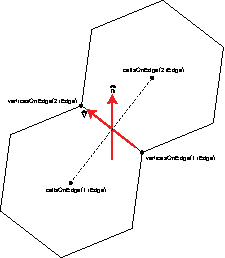
\includegraphics[height=3.5in]{shared/figures/angleEdge.pdf}
\caption{The angle of an edge refers to the angle between a vector pointing north at an edge location
and a vector pointing in the positive tangential velocity direction of the edge.}
\label{fig:angleEdge}
\end{center}
\end{figure}

The angle of each edge in an MPAS grid is provided in the variable {\it angleEdge}. The angle
given is the angle between a vector pointing north and a vector pointing in the
positive tangential direction of the edge. Referring to Fig. \ref{fig:angleEdge},
\[ {\rm angleEdge} = \arcsin\|{\bf \hat n} \times {\bf \hat v}\|, \]
where ${\bf \hat n}$ is the unit vector pointing north and ${\bf \hat v}$ is the unit vector
pointing from verticesOnEdge(1,iEdge) to verticesOnEdge(2,iEdge).

Given a wind vector $(u_\perp, u_\parallel)$ defined in term of components orthogonal to
and parallel to the edge, the earth-relative wind $(u,v)$ may be recovered as
\[
\begin{bmatrix}
u \\
v \\
\end{bmatrix}
=
\begin{bmatrix}
\cos\alpha && -\sin\alpha \\
\sin\alpha && \cos\alpha \\
\end{bmatrix}
\begin{bmatrix}
u_\perp \\
u_\parallel \\
\end{bmatrix},
\]
where $\alpha = {\rm angleEdge}$.




